\documentclass[a4paper,12pt]{article}
\usepackage[english]{babel}
\usepackage[utf8]{inputenc}
\usepackage{amsmath}
\usepackage{amsthm}
\usepackage{amsfonts}
\usepackage{amssymb}
\usepackage{graphicx}
\usepackage{hyperref}
\usepackage{enumitem}
\usepackage{float}
\usepackage{booktabs}
\usepackage{xcolor}
\usepackage{algorithm}
\usepackage{algpseudocode}
\usepackage{CJKutf8}
\usepackage[colorinlistoftodos]{todonotes}
\usepackage[left=1.50cm, right=1.50cm, top=1.20cm]{geometry}
\usepackage{listings}
\usepackage{tikz}
\usetikzlibrary{positioning,arrows,calc, matrix}
\linespread{1.5}


\title{Algorithm Problem Sets \\ \large No. 1 -- 100}
\author{SS}

\begin{document}
\maketitle

\tikzset{
modal/.style={>=stealth',shorten >=1pt,shorten <=1pt,auto,node distance=1.5cm,semithick},
world/.style={circle,draw,minimum size=0.5cm,fill=gray!15},
point/.style={circle,draw,inner sep=0.5mm,fill=black},
reflexive above/.style={->,loop,looseness=7,in=120,out=60},
reflexive below/.style={->,loop,looseness=7,in=240,out=300},
reflexive left/.style={->,loop,looseness=7,in=150,out=210},
reflexive right/.style={->,loop,looseness=7,in=30,out=330}
}

\section{2 -- Add Two Numbers}
You are given two non-empty linked lists $L_1$ and $L_2$ representing two non-negative integers. The digits are stored in reverse order and each of their nodes contain a single digit. Add the two numbers and return it as a linked list.
\par
You may assume the two numbers do not contain any leading zero, except the number 0 itself.
\paragraph{Example:}
\begin{flushleft}
\textbf{Input}:
\begin{figure}[H]
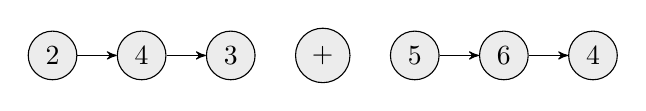
\begin{tikzpicture}
[mynode/.style={circle, draw, minimum size=2mm, fill=gray!15}]
\node(){};
\node(2) [mynode] {2};
\node(4) [mynode, right=5mm of 2] {4};
\node(3) [mynode, right=5mm of 4] {3};
\node(a) [mynode, right=5mm of 3] {$+$};
\node(5) [mynode, right=5mm of a] {5};
\node(6) [mynode, right=5mm of 5] {6};
\node(41) [mynode, right=5mm of 6] {4};
\draw[->,>=stealth'] (2)--(4);
\draw[->,>=stealth'] (4)--(3);
\draw[->,>=stealth'] (5)--(6);
\draw[->,>=stealth'] (6)--(41);
\end{tikzpicture}
\end{figure}
\textbf{Output}
\begin{figure}[H]
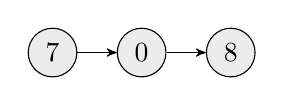
\begin{tikzpicture}
[mynode/.style={circle, draw, minimum size=2mm, fill=gray!15}]
\node(){};
\node(7) [mynode] {7};
\node(0) [mynode, right=5mm of 7] {0};
\node(8) [mynode, right=5mm of 0] {8};
\draw[->,>=stealth'] (7)--(0);
\draw[->,>=stealth'] (0)--(8);
\end{tikzpicture}
\end{figure}
\textbf{Explanation}: $342 + 465 = 807$.
\end{flushleft}


\section{3 --  Longest Substring Without Repeating Characters}
Given a string $S$, find the length of the longest substring without repeating characters.
\paragraph{Example 1:}
\begin{flushleft}
\textbf{Input}: \texttt{abcabcbb}
\\
\textbf{Output}: 3 
\\
\textbf{Explanation}: The answer is \texttt{abc}, with the length of 3. 
\end{flushleft}
\paragraph{Example 2:}
\begin{flushleft}
\textbf{Input}: \texttt{bbbbb}
\\
\textbf{Output}: 1
\\
\textbf{Explanation}: The answer is \texttt{b}, with the length of 1.
\end{flushleft}
\paragraph{Example 3:}
\begin{flushleft}
\textbf{Input}: \texttt{pwwkew}
\\
\textbf{Output}: 3
\\
\textbf{Explanation}: The answer is \texttt{wke}, with the length of 3. Note that the answer must be a substring, \texttt{pwke} is a subsequence and not a substring.
\end{flushleft}
\subsection{Hash Map Approach}
\begin{CJK*}{UTF8}{gbsn}
用一个\texttt{hashmap}来记录每个字符出现的位置,并逐步更新最新的位置。这是因为如果字符$s[j]$在$s[\alpha\ldots j-1]$中在$k$处重复,那么只需要把$\alpha$更新到$k+1$就可以了。
\end{CJK*}
\subsubsection{Code}
Procedure \texttt{GetLongestSubstring} returns the longest slide window for input string $S$.
\begin{algorithm}[H]
\caption{Get longest substring without duplicates}
\begin{algorithmic}[1]
\Procedure{GetLongestSubstring}{$S$}
\State $M$ as $M[0]=\ldots=M[255]:=-1$.
\State $\alpha := 0 $
\State $\beta := 0$ \Comment The maximum length so far
\For{$i := 0$ \textbf{to} $|S|$}
\If{$M(S(i)) \neq -1$} \Comment found repeat $S(i)$ in $S(\alpha\ldots i-1)$
\State $\alpha \gets \max(\alpha, M(S(i))) + 1$ \Comment update to the next index of the duplicate
\EndIf
\State $\beta \gets \max(\beta, i - \alpha +1 )$ \Comment update maximum length so far
\State $M(S(i)) \gets i$ \Comment update $S(i)$ latest index
\EndFor
\State \Return $\beta$
\EndProcedure
\end{algorithmic}
\end{algorithm}

\section{4 --- Median of Two Sorted Arrays}
There are two sorted arrays $A$ and $B$ of size $m$ and $n$ respectively.
\par
Find the median of the two sorted arrays. The overall run time complexity should be $O(\log (m+n))$.
\par
You may assume $A$ and $B$ cannot be both empty.
\paragraph{Example 1:}
\begin{flushleft}
\textbf{Input}: $A = [1, 3]$, $B = [2]$
\\
The median is 2.0
\end{flushleft}
\paragraph{Example 2:}
\begin{flushleft}
\textbf{Input}: $A = [1, 2]$, $B = [3, 4]$
\\
The median is $(2 + 3)/2 = 2.5$
\end{flushleft}
\subsection{Binary Search Approach}
\textbf{\large{Note:}}
\par
\vspace{0.5em}
\begin{CJK*}{UTF8}{gbsn}
\begin{itemize}
\item 假设数组$A$和$B$中,$A[P_A-1]$个和$B[P_B-1]$是处于两个数组合并后处于\texttt{median}处的元素,无论$L_A+L_B$是否为奇偶数,合并后的数组处于$A[P_A-1]$和$B[P_B-1]$之前的元素个数必然是$(L_A+L_B-1)/2$,例如如果$L_A+L_B = 9$,那么\texttt{median}左右的元素个数为$(L_A+L_B-1)/2=4$,因为这时候\texttt{median} 只有一个元素。如果$L_A+L_B = 10$,那么这时候\texttt{median}有两个元素,但是这两个元素的左右两边的元素个数仍然为$(L_A+L_B-1)/2=4$,不同的只是这时候\texttt{median}是两个元素。至于$A[P_A-1]$和$B[P_B-1]$谁是\texttt{median}还是两者都是,没有关系。
\item 根据上述分析,就可以得到$P_A-1+P_B-1 =(L_A+L_B-1)/2 $,变换一下形式,得到如下关系
\[
P_A + P_B = (L_A+L_B+1)/2
\]
\item 采用二分法查询在数组A中的$P_A$位置,使得上述关系成立,同时还需要有以下关系
\[
A[P_A - 1] \leq B[P_B] \quad \mathtt{and} \quad B[P_B - 1] \leq A[P_A]
\]
这是因为$A[P_A-1]$个和$B[P_B-1]$是处于两个数组合并后处于\texttt{median}处的元素,如果不能满足以上关系,$A[P_A-1]$个或者$B[P_B-1]$就不再是处于\texttt{median}处的元素了。
\item 由于$P_A$的取值范围是$0\to L_A$,所以$P_B$的取值范围就是$(L_B-L_A+1)/2 \to (L_A+L_B+1)/2$。为了保证$P_B$的最小值仍然大于等于0,可以强制设定$L_B$为$A$, $B$中的较长数组。
\end{itemize}
\end{CJK*}
\subsubsection{Code}
Procedure \texttt{FindMedian} returns the median value of $A$ and $B$ with size $m$ and $n$ respectively.
\setcounter{algorithm}{0}
\begin{algorithm}[H]
\caption{Binary Search Approach}
\begin{algorithmic}[1]
\Procedure{FindMedian}{$A, m, B, n$}
\State $\ell: = (m + n + 1)/2$ \Comment set half length for the merged array
\If{$m > n$}
\State \textbf{swap} $A$ and $B$ \Comment make sure $B$ is the \textbf{longer} array
\EndIf
\State $l := 0$ and $r:=m$ \Comment Start binary search
\While{$l \leq r$}
\State $P_A := (l+r)/2$ \Comment get middle point in $A$
\State $P_B := \ell - P_A$ \Comment get number of elements need to be from $B$
\If{$P_A > 0 $ \textbf{and} $A[P_A-1] > B[P_B]$ }
\State $r \gets P_A -1 $ \Comment Search in the lower half
\ElsIf{$P_A < L_A $ \textbf{and} $ A[P_A] < B[P_B-1]$}
\State $l \gets P_A +1 $ \Comment Search in the upper half
\Else
\If{$P_A=0$}
\State $\theta_1 := B[P_B-1]$ \Comment No element from $A$ below than \textbf{median}
\ElsIf{$P_B = 0$}
\State $\theta_1 := A[P_A-1]$ \Comment No element from $B$ below than \textbf{median}
\Else 
\State $\theta_1 := \max(A[P_A - 1], B[P_B-1])$ \Comment The lower median is the greater one
\EndIf
\If{$P_A = m$}
\State $\theta_2 := B[P_B]$ \Comment all elements from $A$ below than \textbf{median}
\ElsIf{$P_B = n$}
\State $\theta_2 := A[P_A]$ \Comment all elements from $B$ below than \textbf{median}
\Else
\algstore{myalg}
\end{algorithmic}
\end{algorithm}

\begin{algorithm}[H]
\begin{algorithmic}[1]
\algrestore{myalg}
\State $\theta_2 := \min(A[P_A], B[P_B])$ \Comment The lower median is the \textbf{smaller} one
\EndIf
\EndIf
\If{$(m+n) \bmod 2 = 0$} \Comment even length
\State \Return $(\theta_1 + \theta_2)/2$
\Else \Comment odd length
\State \Return $\theta_1$
\EndIf
\EndWhile
\EndProcedure
\end{algorithmic}
\end{algorithm}

\section{5 -- Longest Palindromic Substring}
Given a string $S$, find the longest palindromic substring in $S$. You may assume that the maximum length of $s$ is 1000.
\paragraph{Example 1:}
\begin{flushleft}
\textbf{Input}: \texttt{babad}
\\
\textbf{Output}: \texttt{bab}
\\
\textbf{Note}:  \texttt{aba} is also a valid answer.
\end{flushleft}
\paragraph{Example 2:}
\begin{flushleft}
\textbf{Input}: \texttt{cbbd}
\\
\textbf{Output}: \texttt{bb}
\end{flushleft}
\subsection{Dynamic Programming Approach}
\begin{CJK*}{UTF8}{gbsn}
方法一: \texttt{Dynamic Programming}. \texttt{DP}方法也有两种,以长度为循环条件,以及倒序推。两种方法的\texttt{DP}公式一样
\[
DP[i][j]  = 
\begin{cases}
 0 & \iff S[i] \neq S[j] \\
 DP[i+1][j-1] &\iff S[i] = S[j]
\end{cases}
\]
\par
这两种\texttt{DP}所需的空间复杂度都为$O(n^2)$,但是第二种方法可以做进一步修改,使得空间复杂度为$O(n)$
\par
方法二: 由于只有一维数组,所以数组中的每个元素在循环中都要被更新而不是固定不变,这点是和二维\texttt{DP}不同的地方。
\end{CJK*}
\subsubsection{Code}
Procedure \texttt{LongestPalindrome} returns the longest palindrome string for input string $S$.
\setcounter{algorithm}{0}
\begin{algorithm}[H]
\caption{\texttt{DP} Method 1: loop by substring length}
\begin{algorithmic}[1]
\Procedure{LongestPalindrome}{$S$}
\State \texttt{DP} := \textbf{boolean array} with $|S|\times|S|$
\State $L_\mathtt{max} := 1$ \Comment maximum palindrome length is initialized with \textbf{1} 
\For{$i:=0$ \textbf{to} $|S|-1$}
\State $\mathtt{DP}[i][i] \gets 1$ \Comment single character is \textbf{palindrome} by itself.
\EndFor
\For{$l:=2$ \textbf{to} $|S|$} \Comment substring length from $2 \to |S|$
\For{$i := 0$ \textbf{to} $|S| - l$} \Comment the start of substring is from $0 \to |S| - l$
\State $j := i + l - 1$ \Comment the end of substring
\If{$S[i] \neq S[j]$}
\State $\mathtt{DP}[i][j] = 0$ \Comment $S[i\ldots j] $cannot be \textbf{palindrome}
\Else
\State $\mathtt{DP}[i][j] = \mathtt{DP}[i+1][j-1]$ 
\EndIf
\If{$\mathtt{DP}[i][j] = \mathtt{true}$} \Comment $S[i\ldots j]$ is \textbf{palindrome}
\If{$L_\mathtt{max} < l$}
\State $S_\mathtt{max} := S[i\ldots j]$ \Comment update \textbf{longest palindrome} as $S[i\ldots j]$
\State $L_\mathtt{max} \gets l$ \Comment update \textbf{maximum palindrome length}
\EndIf
\EndIf
\EndFor
\EndFor
\State \Return $S_\mathtt{max}$
\EndProcedure
\end{algorithmic}
\end{algorithm}

\begin{algorithm}[H]
\caption{\texttt{DP} Method 2: backward}
\begin{algorithmic}[1]
\Procedure{LongestPalindrome}{$S$}
\State \texttt{DP} := \textbf{1 dimension array} with $\mathtt{size} = |S|$ and all elements are \textbf{false}
\State $L_\mathtt{max} := 1$ \Comment maximum palindrome length is initialized with \textbf{1} 
\For{$i:=|S|-1$ \textbf{to} $0$}
\For{$j:=|S|-1$ \textbf{to} $i$}
\If{$S[i] \neq S[j]$}
\State $\mathtt{DP}[j] \gets \mathtt{false}$ \Comment Update $\mathtt{DP}[j]$ in each loop although it is \textbf{true} in previous loop
\Else
\If{$j-i\leq 2$}
\State $\mathtt{DP}[j] \gets \mathtt{true}$ \Comment If substring length $\leq 2$, directly update $\mathtt{DP}[j]$
\Else 
\State $\mathtt{DP}[j] \gets \mathtt{DP}[j-1]$ \Comment  Update $\mathtt{DP}[j]$ as $\mathtt{DP}[j-1]$ 
\EndIf
\EndIf
\If{$\mathtt{DP}[j] = \mathtt{true}$} \Comment Found palindrome
\If{$j-i +1 > L_\mathtt{max}$} \Comment Found maximum palindrome so far
\State $L_\mathtt{max} \gets j-i +1$
\State $S_\mathtt{max} \gets S[i\ldots j]$
\EndIf
\EndIf
\EndFor
\EndFor
\State \Return $S_\mathtt{max}$
\EndProcedure
\end{algorithmic}
\end{algorithm}


\section{6 --- ZigZag Conversion}
The string \texttt{PAYPALISHIRING} is written in a zigzag pattern on a given number of rows like this: 
\begin{table}[H]
\begin{tabular}{lllllll}
P &   & A &   & H &   & N \\
A & P & L & S & I & I & G \\
Y &   & I &   & R &   &  
\end{tabular}
\end{table}
And then read line by line: \texttt{PAHNAPLSIIGYIR}
\par
Write the code that will take a string $S$ and make this conversion given a number of rows $N$:
\paragraph{Example 1:}
\begin{flushleft}
\textbf{Input}: $S = \texttt{PAYPALISHIRING}$, $ N = 3$
\\
\textbf{Output}: \texttt{PAHNAPLSIIGYIR}
\\
\textbf{Explanation}:
\end{flushleft}
\begin{table}[H]
\begin{tabular}{lllllll}
P &   &   & I &   &   & N \\
A &   & L & S &   & I & G \\
Y & A &   & H & R &   &   \\
P &   &   & I &   &   &  
\end{tabular}
\end{table}

\subsection{Visit By Row}
Visit all characters in row 0 first, then row 1, then row 2, and so on\dots
\par
\begin{itemize}
\item Characters in row $0$ are located at indexes $0, \left(2 \times N - 2\right), 2\times\left(2 \times N - 2\right), \ldots$
\item Characters in row $N-1$ are located at indexes $N-1, \left(2 \times N - 2\right) + N - 1, 2\times\left(2 \times N - 2\right) + N - 1, \ldots$
\item Characters in inner row $0<i<N-1$ are located at indexes 
\[
i, \left(2 \times N - 2\right)-i, \left(2 \times N - 2\right) + i, 2\times\left(2 \times N - 2\right)- i, 2\times\left(2 \times N - 2\right)+ i, 3\times\left(2 \times N - 2\right)- i, \dots
\]
\end{itemize}
\setcounter{algorithm}{0}
\begin{algorithm}[H]
\caption{Print letters in Zigzag way}
\begin{algorithmic}[1]
\Statex
\Procedure{Zigzag}{$S, L, N$}
\If{$N = 1$}
\State \Return $S$ \Comment one row is $S$ itself
\EndIf
\State $\delta := 2 \times N -2$
\State $Z:= \emptyset$ \Comment $Z$ will be the print string
\For{$n:=0$ \textbf{to} $N-1$}
\State $k:= 0$
\While{$k+n < L$}
\State $Z \gets Z + S[k+n]$ \Comment $S[m\times \left(2 \times N - 2\right)] + i$ for $m = 1,2, \ldots$ and $i = 0, \ldots, N-1$
\If{$n\neq 0$ \textbf{and} $n\neq N-1$ \textbf{and} $k+\delta - n < L$} \Comment For inner rows
\State $Z \gets Z + S[k+\delta-n]$ \Comment get $S[m\times\left(2 \times N - 2\right)- i]$
\EndIf
\State $k \gets k+\delta$
\EndWhile
\EndFor
\State \Return $Z$
\EndProcedure
\Statex
\end{algorithmic}
\end{algorithm}

\section{7 --- Reverse Integer}
Given a 32-bit signed integer $N$, reverse digits of an integer.
\paragraph{Example 1:}
\begin{flushleft}
\textbf{Input}: 123
\\
\textbf{Output}: 321
\end{flushleft}
\paragraph{Example 2:}
\begin{flushleft}
\textbf{Input}: $-123$
\\
\textbf{Output}: $-321$
\end{flushleft}
\paragraph{Example 3:}
\begin{flushleft}
\textbf{Input}: 120
\\
\textbf{Output}: 21
\end{flushleft}
\paragraph{Note:}
Assume we are dealing with an environment which could only store integers within the 32-bit signed integer range: $[-2^{31}, 2^{31}-1]$. For the purpose of this problem, assume that your function returns 0 when the reversed integer overflows.
\subsection{Intuition}
We can build up the reverse integer one digit at a time. While doing so, we can check beforehand whether or not appending another digit would cause overflow.
\begin{itemize}
\item Reversing an integer can be done similarly to reversing a string.
\item We want to repeatedly \textbf{pop} the last digit off of $x$ and \textbf{push} it to the back of the $\mathbf{R}$. In the end, $\mathbf{R}$ will be the reverse of the $x$.
\item To \textbf{pop} and \textbf{push} digits without the help of some auxiliary stack/array
\begin{itemize}
\item \textbf{pop}: 

\begin{align*}
\mathtt{pop} &= x \bmod 10 \\
x &= \frac{x}{10}
\end{align*}

\item \textbf{push}:
\begin{align*}
T &= R \times 10 + \mathtt{pop} \\
R &= T
\end{align*}
\end{itemize}
\item However, $T$ could be overflow, Suppose $I_{\max}$ is the maximum value represented by integer type.
\begin{enumerate}
\item if $T = R \times 10 + \mathtt{pop}$ has overflow, it must be $R \geq \dfrac{I_{\max}}{10}$
\item if $R > \dfrac{I_{\max}}{10} $, $T$ will be overflow for sure.
\item if $R = \dfrac{I_{\max}}{10}$, $T$ will be overflow $\iff \mathtt{pop} > 7$, because $I_{\max} = 2^{31} - 1 = 2147483647$
\end{enumerate}
\item similar when $R$ is underflow, and $I_{\min} = -2^{31} = -2147483648$
\end{itemize}

\setcounter{algorithm}{0}
\begin{algorithm}[H]
\caption{Reverse an integer}
\begin{algorithmic}[1]
\Statex
\Procedure{ReverseInteger}{$N$}
\State $R:=0$ \Comment $R$ is the result of reverse
\State $R_{\max}:= \dfrac{I_{\max}}{10}$ \Comment threshold for $R$ to avoid overflow
\State $R_{\min}:= \dfrac{I_{\min}}{10}$ \Comment threshold for $R$ to avoid underflow
\While{$N \neq 0$}
\State $\mathtt{pop} := N \bmod 10$
\State $N = \dfrac{N}{10}$
\If{$R > R_{\max}$ \textbf{or} ($R=R_{\max}$ \textbf{and} $\mathtt{pop} > 7$)} \Comment overflow
\State \Return 0
\ElsIf{$R < R_{\min}$ \textbf{or} ($R=R_{\min}$ \textbf{and} $\mathtt{pop} < -8$)} \Comment underflow
\State \Return 0
\Else
\State $R\gets R\times 10 + \mathtt{pop}$
\EndIf
\EndWhile
\EndProcedure
\Statex
\end{algorithmic}
\end{algorithm}

\section{9 --- Palindrome Number}
Determine whether an integer $N$ is a palindrome. An integer is a palindrome when it reads the same backward as forward.
\paragraph{Example 1:}
\begin{flushleft}
\textbf{Input}: 121
\\
\textbf{Output}: 1
\\
\textbf{Explanation}:
\end{flushleft}
\paragraph{Example 2:}
\begin{flushleft}
\textbf{Input}: $-121$
\\
\textbf{Output}: 0
\\
\textbf{Explanation}:
\\
From left to right, it reads $-121$. From right to left, it becomes $121-$. Therefore it is not a palindrome.
\end{flushleft}
\paragraph{Example 3:}
\begin{flushleft}
\textbf{Input}: 10
\\
\textbf{Output}: 0
\\
\textbf{Explanation}:
\\
Reads 01 from right to left. Therefore it is not a palindrome.
\end{flushleft}
\subsection{Revert half of the number}
\begin{itemize}
\item The first idea that comes to mind is to convert the number into string, and check if the string is a palindrome, but this would require extra non-constant space for creating the string which is not allowed by the problem description.
\item Second idea would be reverting the number itself, and then compare the number with original number, if they are the same, then the number is a palindrome. However, if the reversed number is larger than $2^{32}$, it causes integer overflow.
\item Following the thoughts based on the second idea, to avoid the overflow issue of the reverted number, what if revert {\color{red}half} of the number? After all, the reverse of the last half of the palindrome should be the same as the first half of the number, if the number is a palindrome.
\par
For example, if the input is 1221, if we can revert the last part of the number \textbf{1221} from {\textbf{\color{blue}21}} to {\textbf{\color{red}12}}, and compare it with the first half of the number \textbf{12}, since 12 is the same as 12, we know that the number is a palindrome.
\end{itemize}
\subsubsection{Code}
Procedure \texttt{IsPalindrome} check if $N$ is a palindrome. If it is, the procedure returns 1. Otherwise, it returns 0. We could have the following observations.
\begin{itemize}
\item All {\color{red}negative} numbers are not palindrome, for example: $-123$ is not a palindrome since the $-$ does not equal to $3$. 
\item All multiply of \textbf{10} are not palindrome. The first number cannot be {\color{red}0}
\item How to know reaching the {\color{red}half} of the number? Since the number is divided by 10, and the reversed number is multiplied by 10, when the original number is {\color{red}less than} the reversed number, it means we've processed half of the number digits.
\item If the number length is odd, such as \textbf{12321}. When loop ended, the reversed number will be $12$, while origin number becomes $123$. Therefore, need to check if $12 = \dfrac{123}{10}$
\end{itemize}
\setcounter{algorithm}{0}
\begin{algorithm}[H]
\caption{Check if the integer is a palindrome number}
\begin{algorithmic}[1]
\Statex
\Procedure{IsPalindrome}{$N$}
\If{$N < 0$ \textbf{or} $N \bmod 10 \equiv 0$} \Comment {{\color{red}negative}} or multiply of \textbf{10} cannot be palindrome number
\State \Return 0
\EndIf
\State \textbf{$R := 0$} \Comment $R$ is the \textbf{reversed number}
\While{$N > R$} \Comment check if reaching to half of $N$
\State $q := N\div 10$
\State $r := N\bmod 10$
\State $R \gets R\times 10 + r$
\State $N\gets q$ \Comment Update $N$
\EndWhile
\If{$N \neq R$ \textbf{and} $N \neq \dfrac{R}{10}$} \Comment {{\color{red}cannot}} be palindrome number
\State \Return 0
\Else
\State \Return 1
\EndIf
\EndProcedure
\Statex
\end{algorithmic}
\end{algorithm}

\section{10 --- Regular Expression Matching}
Given an input string $S$ and a pattern $P$, implement regular expression matching with support for $(.)$ and $(\ast)$.
\begin{itemize}
\item $(.)$ Matches any single character.
\item $(\ast)$ Matches zero or more of the preceding element.
\end{itemize}
The matching should cover the entire input string (not partial).
\paragraph{Note:}
\begin{itemize}
\item $S$ could be empty and contains only lowercase letters a--z.
\item $P$ could be empty and contains only lowercase letters a--z, and characters like $(.)$ or $(\ast)$.
\end{itemize}
\paragraph{Example 1:}
\begin{flushleft}
\textbf{Input}: $S=\texttt{aa}$, $P=\texttt{a}$
\\
\textbf{Output}: 0
\\
\textbf{Explanation}: \texttt{a} does not match the entire string \texttt{aa}.
\end{flushleft}
\paragraph{Example 2:}
\begin{flushleft}
\textbf{Input}: $S=\texttt{aa}$, $P=\texttt{a}\ast$
\\
\textbf{Output}: 1
\\
\textbf{Explanation}:
\\
$(\ast)$ means zero or more of the preceding element, \texttt{a}. Therefore, by repeating \texttt{a} once, it becomes \texttt{aa}.
\end{flushleft}
\paragraph{Example 3:}
\begin{flushleft}
\textbf{Input}: $S=\texttt{ab}, P=.\ast$
\\
\textbf{Output}:
\\
\textbf{Explanation}:
\\
$.\ast$ means zero or more ($\ast$) of any character ($.$).
\end{flushleft}
\paragraph{Example 4:}
\begin{flushleft}
\textbf{Input}: $S = \texttt{aab}, P = \texttt{c}\ast\texttt{a}\ast\texttt{b}$
\\
\textbf{Output}: 1
\\
\textbf{Explanation}:
\\
$c$ can be repeated 0 times, a can be repeated 1 time. Therefore it matches \texttt{aab}.
\end{flushleft}
\paragraph{Example 5:}
\begin{flushleft}
\textbf{Input}: $S = \texttt{mississippi}$, $P = \texttt{mis}\ast\texttt{is}\ast\texttt{p}\ast$
\\
\textbf{Output}: 0
\end{flushleft}

\subsection{Recursive Approach}
Notice that {\color{red}$\ast$} can not be the first character of pattern because it relates to the {\color{red}preceding} element.
\begin{itemize}
\item If there were no {\color{red}$\ast$}, just check from left to right if each character of the $S$ matches $P$.
\item If a {\color{red}$\ast$} is present in $P$, it will be in the \textbf{\color{red}2nd} position i.e. $P[1]$. 
\begin{itemize}
\item Suppose $\ast$ means one ore more $P[0]$, if $S[0]=P[0]$, $P[0]$ will still be there. therefore need to check $S[1\ldots]$ and $P[0]$.
\item Suppose $\ast$ means nothing. Therefore, $P[0]$ does not exist, need to check $S[0\ldots]$ and $P[2]$.
\end{itemize}
\end{itemize}

Procedure \texttt{IsMatch} check if input string $S$ with length $L$ matches pattern string $P$ with length $M$. 

\setcounter{algorithm}{0}
\begin{algorithm}[H]
\caption{Regex match using recursive method}
\begin{algorithmic}[1]
\Procedure{IsMatch}{$S, L, P, M$}{\label{010match}}
\If{$P = \emptyset$} \Comment pattern $P$ is empty
\If{$S = \emptyset$}
\State \Return \textbf{\color{red}True} \Comment Only if $S$ is be empty, $S$ and $P$ can be matched.
\Else
\State \Return \textbf{False}
\EndIf
\EndIf
\State $M_{0} :=$ False 
\If{$S \neq \emptyset$ \textbf{and} ( $S[0] = P[0]$ \textbf{or} $P[0] = \cdot$ ) } \Comment check if the first character is matched
\State $M_{0} :=$ \textbf{\color{red}True}
\EndIf
\State $M_{1} :=$ False
\If{$L_{P} \geq 2$ \textbf{and} $P[1] = \ast$} \Comment check if there is a $\ast$ in $P[1]$
\State $M_{1} :=$ \textbf{\color{red}True}
\EndIf
\If{$M_{1}$ \textbf{is} \textbf{\color{red}True}} \Comment $P[1] = \ast$
\If{\texttt{IsMatch}($S[0\ldots]$, $P[2\ldots]$) \textbf{is} \textbf{\color{red}True}} \Comment recursive call \ref{010match}
\State \Return \textbf{True} 
\ElsIf{($M_{0}$ is \textbf{\color{red}True}) \textbf{and} ($S\neq \emptyset$) \textbf{and} (\texttt{IsMatch}($S[1\ldots]$, $P[0\ldots]$)}
\State \Return \textbf{True} 
\EndIf
\Else \Comment $P[1] \neq \ast \rightarrow$ match one by one
\If{($M_{0}$ is \textbf{\color{red}True}) \textbf{and} ($S\neq \emptyset$) \textbf{and} (\texttt{IsMatch}($S[1\ldots]$, $P[1\ldots]$)} \Comment recursive call \ref{010match}
\State \Return \textbf{True}
\EndIf
\EndIf
\State \Return \textbf{False} \Comment Cannot get match
\EndProcedure
\end{algorithmic}
\end{algorithm}

\subsection{Dynamic Programming}
As the problem has an optimal substructure, it is natural to cache intermediate results. Suppose the recursive function $F(i, j)$ will tell us if $S[i\ldots L-1]$ and $P[j\ldots m-1]$ match.
\par
We proceed with the same recursion as above approach, except that when to match $S[i\ldots L-1]$ with $P[j\ldots m-1]$, we can use memorized intermediate result $F(i, j)$.
\begin{algorithm}[H]
\caption{Top Down Dynamic Programming}
\begin{algorithmic}[1]
\Procedure{IsMatch}{$S, L, P, M$}
\State $F$ as $F[0][0] = \ldots = F[L][M]:=-1$ \Comment F is $(L+1)\times(M+1)$ array
\State $\gamma:=\Gamma(S, L, P, M, 0, 0, F)$ \Comment Start with $i=0$ and $j=0$
\State \Return $\gamma$
\EndProcedure
\end{algorithmic}
\end{algorithm}

Function $\Gamma$ check if $S$ matches with $P$ starting with $S[i]$ and $P[j]$ using $F$ as memo array. The match results is $1/0$.

\begin{algorithm}[H]
\caption{Top Down Dynamic Programming}
\begin{algorithmic}[1]
\Function{$\Gamma$}{$S, L, P, M, i, j, F$}
\If{$F[i][j] \neq -1$}
\State \Return $F[i][j]$ \Comment Return $F[i][j]$ if it has been already memorized
\EndIf
\State $\mu:=0$ \Comment The match result
\If{$j = M$} \Comment $P$ is completely scanned \label{10if1}
\If{$i=L$}
\State $\mu\gets 1$ \Comment $S$ matches $P$
\Else
\State $\mu\gets0$ \Comment $S$ does not match $P$
\EndIf
\State $\beta:=0$ \Comment $0/1$ variable to indicate if $S[i]$ matches $P[j]$

\If{$i<L$} \label{10if2}
\If{$S[i] = P[j]$}
\State $\beta \gets 1$
\ElsIf{$P[j]=(.)$} \Comment dot matches one character

\algstore{10gamma}
\end{algorithmic}
\end{algorithm}
\begin{algorithm}[H]
\begin{algorithmic}[1]
\algrestore{10gamma}
\State $\beta \gets 1$
\EndIf
\EndIf \Comment End[\ref{10if2}]

\If{$j+1< M$ \textbf{and} $P[j+1]=(\ast)$} $(\ast)$ can match zero or more $P[j]$ \label{10if3}
\State $\mu \gets \Gamma(S,L,P,M,i, j+2, F)$ \Comment $\ast$ ignore $P[j]$, check $S[i\ldots]$ with $P[j+2\ldots]$
\If{$\mu \neq 1$} \Comment $S[i]$ does not match $P[j+2\ldots]$ \label{10if4}
\If{$\beta=1$} \Comment $S[i]$ match $P[j]$
\State $\mu \gets \Gamma(S,L,P,M,i+1, j, F)$ \Comment $\ast$ is one $P[j]$, check $S[i+1\ldots]$ to $P[j\ldots]$
\EndIf 
\EndIf \Comment End[\ref{10if4}]
\Else
\If{$\beta=1$} \Comment $S[i]$ match $P[j]$
\State $\mu\gets \Gamma(S,L,P,M,i+1, j+1, F)$ \Comment Check $S[i+1\ldots]$ with $P[j+1\ldots]$
\EndIf 
\EndIf \Comment End[\ref{10if3}]
\EndIf \Comment End[\ref{10if1}]
\State $F[i][j] \gets \mu$ \Comment Memorize the result
\State \Return $\mu$
\EndFunction
\end{algorithmic}
\end{algorithm}

\end{document}
